\chapter{Conclusion et Perspectives}

\minitoc

\section{Résumé de cette thèse}

L'objectif principal de cette thèse était de comprendre l'influence d'une couche de matériau granulaire le long d'une interface frictionnelle sur la dynamique de glissement d'une faille de laboratoire. Afin d'éclaircir cette problématique, nous l'avons introduite à l'aune de plusieurs domaines de la physique, la mécanique des frottements, la mécanique de la fracture et la mécanique des failles, ayant chacune leur approche et leur description des systèmes frictionnels désordonnés (Chap.\,\ref{sec:chapintro}).

Cette thèse s'inscrit dans une démarche expérimentale, portée par le développement au cours de notre étude d'un dispositif mécanique, électronique et optique polyvalent adapté à l'étude des interfaces frictionnelles, en particulier en présence de milieu granulaire (Chap.\,\ref{sec:chapxp}).
\begin{itemize}
\bitem Le dispositif mécanique est une presse motorisée polyvalente, réalisée en partenariat avec le Service d'Ingénierie Mécanique de l'ENS de Lyon, permettant de presser et cisailler des plaques minces, formant une interface frictionnelle.
\bitem Les blocs formant l'interface étudiée ont été densément équipés de capteurs de déformations. Ces capteurs permettent une mesure à \SI{4}{\mega\hertz} du tenseur des déformations en 20 points le long de l'interface, et la détection de la propagation de ruptures frictionnelles lors de l'initiation du mouvement de glissement. Ces capteurs sont conditionnés électroniquement par un amplificateur de précision réalisé durant la thèse en partenariat avec le Service d'Ingénierie Électronique du Laboratoire de Physique à l'ENS de Lyon.
\bitem Les grains, marqués d'un motif reconnaissable, sont suivis par imagerie. Leur position est déterminée à une résolution micrométrique au moyen d'un algorithme de suivi sous-pixel par corrélation d'images.
\end{itemize}

Au moyen de ce dispositif nous avons pu effectuer un travail préliminaire sur les interfaces entièrement granulaires, et avons tout particulièrement approfondi l'étude de la dynamique d'une interface en œil granulaire (Chap.\,\ref{sec:chaparticle}). Il s'agit d'une interface solide-solide perturbée par l'inclusion sur une portion de sa longueur d'un milieu granulaire dense, encapsulé dans les blocs sous la forme d'un œil. Nous avons étudié l'influence de la densité du milieu granulaire sur la dynamique macroscopique et locale du système, et avons abouti à l'établissement d'un mécanisme par lequel l'œil granulaire déstabilise l'interface et la mène à glisser prématurément en comparaison avec une interface solide-solide dans les mêmes conditions de chargement.

\pagebreak

Le mécanisme que nous avons observé est le suivant :
\begin{itemize}
\bitem L'œil granulaire entraîne une augmentation de la fréquence de stick-slip de l'interface. Cette augmentation est d'autant plus grande que le milieu granulaire est dense
\bitem Un patch glissant apparaît à l'interface. Ce patch s'étend et glisse entre les évènements sismiques, d'autant plus que le milieu granulaire est dense.
\bitem Le patch agit alors comme un crack de Griffith en mode de cisaillement, se déstabilisant à une contrainte cisaillante macroscopique d'autant plus faible que sa longueur est grande.
\end{itemize}
Ce mécanisme enrichi la diversité des phénomènes observés le long des interfaces fictionnelles hétérogènes (Chap.\,\ref{chap:etatdelart}). Notre étude effectue un lien entre la mécanique de la fracture frictionnelle et la mécanique des failles, et participe à l'éclaircissement des mécanismes à l'origine des séismes lents, et de leurs interactions avec les zones sismiques. Elle met en particulier en évidence un mécanisme par lequel un patch glissant, pouvant être associé à une portion de faille au frottement renforcé par la vitesse, peut participer au déchargement par des séismes de faible amplitude de portions de faille éloignées, affaiblies par la vitesse. L'évolution de l'extension spatiale de la zone en glissement lent pourrait être un facteur clé dans la compréhension des mécanismes de co-sismicité dans les failles réelles.




\section{Perspectives}


Notre étude et le développement du dispositif expérimental que nous présentons dans cette thèse ouvrent la voie à de nouvelles perspectives prometteuses pour l'étude d'interfaces granulaires cisaillées. En effet l'objectif initial de cette thèse était l'étude d'une interface entièrement granulaire, mais celle-ci s'est avérée nécessiter un équipement dont nous ne disposions pas alors. Munis de ce dispositif, et forts de ces résultats sur les interfaces hétérogènes, nous pouvons revenir à ces problématiques, et en aborder de nouvelles.


\subsection{Interface hétérogène}

L'interface en œil granulaire est un exemple d'interface hétérogène dans laquelle l'hétérogénéité agit comme une hétérogénéité de contrainte créant un patch glissant. Modifier la nature de l'hétérogénéité nous permettrait d'approfondir nos connaissances sur les mécanismes liées à ces interfaces. Dans le cas de l'œil, la fonction du milieu granulaire de créer un patch glissant pourrait être remplie par d'autres milieux, soit granulaires de propriétés différentes, soit solides sous la forme d'une inclusion d'un matériau différent ou de forme différente. Nous pourrions ainsi déterminer les contributions de chaque paramètre de l'étude indépendamment.

De plus le milieu granulaire choisi est particulièrement glissant, puisque la friction entre les grains de nylon est relativement faible en raison de leur état de surface créé par extrusion. L'augmentation de la rugosité de ceux-ci, l'utilisation de matériaux différents, ou de géométries de grains différentes, sont des développements envisagés pour le futur proche.

Enfin l'instrumentation électronique développée au cours de la thèse étant désormais opérationnelle, il serait possible d'instrumenter les blocs de manière plus dense et de répliquer cette étude avec une mesure plus fine du tenseur des déformations à l'interface.

Le développement électronique que nous avons effectué nous permet également de reprendre l'étude de l'interface entièrement granulaire.

\subsection{Dynamique d'une interface entièrement granulaire}
\label{sec:fullygranpersp}

\begin{figure}[phtb]
\centering
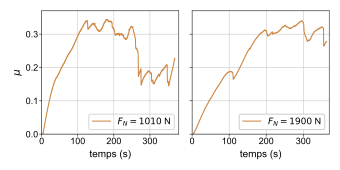
\includegraphics[scale=1]{../Figures_chap_conclusion/fullygran.pdf}
\caption[Dynamique locale d'une interface entièrement granulaire]{Exemples d'évolution de $\mu=F_S/F_N$ lors de deux expériences entièrement granulaires. L'interface est alors en glissement permanent, ponctué d'évènements rapides de relâchement des contraintes.}
\label{fig:dyngran}
\end{figure}

\begin{figure}[phtb]
\centering
\includegraphics[scale=1]{../Figures_chap_conclusion/difference.pdf}
\caption[Dynamique locale d'une interface entièrement granulaire]{Exemple d'évènements rapides dans une interface entièrement granulaire. Les trois images de chaque sous-figure correspondent respectivement à une image prise quelques millisecondes avant l'évènement, une image quelques millisecondes après l'évènement, et la différence entre les deux images. Les différences sont également signalées en rouge sur les images avant-après. \textbf{a.}\,Évènement de glissement total de l'interface. \textbf{b.}\,Évènement de réarrangement local des grains à l'interface.}
\label{fig:dyngranlocal}
\end{figure}


Lorsqu'une expérience de cisaillement est menée sur une interface entièrement granulaire, celle-ci peut exhiber différentes dynamiques macroscopiques. Lorsque la couche granulaire est épaisse de quelques grains, nous avons tout particulièrement observé un mouvement de glissement permanent, ponctué d'évènements de glissement rapide (Fig.\,\ref{fig:dyngran}). Le glissement, rapide ou lent, est associé à un réarrangement des grains. Lorsque le glissement est lent, ceux-ci glissent les uns sur les autres, et sont en frottement dynamique. Lorsque le réarrangement est rapide, l'interface est dans une configuration bloquée géométriquement, dans laquelle cisailler les grains nécessite de dilater le milieu granulaire, et donc d'augmenter l'énergie potentielle élastique des blocs. Cette énergie élastique est alors relâchée de manière brutale par un réarrangement rapide des grains (Fig.\,\ref{fig:dyngranlocal}). Ces réarrangements peuvent être locaux ou généralisés.

Une hypothèse sur la dynamique de ces réarrangements est qu'ils sont initialement médiés par une rupture, mais que nous n'observons que les effets de la mise en glissement inertiel de l'interface. Ces ruptures peuvent de plus être arrêtées en raison de la forte hétérogénéité de la distribution des contraintes normales $\sigma_{yy}(x)$, et donc de l'énergie de fracture $\Gamma\propto\sigma_{yy}$. Une autre hypothèse serait que la zone de nucléation est plus grande que la taille de notre interface.

Notre objectif expérimental est désormais de trouver des conditions expérimentales permettant d'atteindre un mouvement de stick-slip. Les pistes que nous envisageons pour atteindre cet objectif sont soit d'augmenter la densité du milieu granulaire en ajoutant des cylindres plus fins pour combler les interstices, soit de jouer sur la géométrie des grains afin de les bloquer géométriquement.

Nous sommes maintenant équipés d'un dispositif de mesure alliant une grande densité de jauges de déformations et une imagerie rapide. Les jauges nous permettent de mesurer le passage du front de rupture, et d'étudier le déplacement associé. La caméra nous permet de suivre avec précision les grains à l'interface, d'autant que zoomer sur une portion de l'interface augmente la résolution du suivi et la vitesse d'acquisition.





\subsection{Étude statistique par mesures acoustiques}


L'étude des interfaces entièrement granulaires ne se limite pas à celle de leur dynamique locale, mais peut se rapprocher de celle d'une faille sismique réelle. En effet la disparité des tailles des évènements de réarrangement rapide des grains nous laisse à penser que le système pourrait se comporter comme une faille réelle, et vérifier une loi de Gutenberg-Richter (Sec.\,\ref{sec:failles}). Cette hypothèse est renforcée par l'existence d'études montrant qu'un milieu granulaire cisaillé par des plaques infiniment rigides reproduit cette loi\,\cite{lherminier_continuously_2019, geller_stick-slip_2015, ramos_avalanche_2009, houdoux_micro-slips_2021} (Chap.\,\ref{chap:etatdelart}).

Dans l'objectif d'étudier cette hypothèse, nous collaborons avec l'équipe de sismologie de Thomas Bodin, Stéphanie Durand, Blandine Gardonio et Marine Laporte au Laboratoire de Géologie de Lyon (LGLTPE), ainsi qu'Osvanny Ramos de l’Institut Lumière Matière de Lyon (ILM). L'objectif de cette collaboration est de faire le lien entre des observations sismiques de terrain et des expériences en laboratoire.

Les catalogues sismiques accumulés depuis le premier enregistrement de séisme en 1984 sont une manne d'informations importante, permettant de mieux comprendre les mécanismes de la sismicité. Leur étude a mené à l'élaboration de lois empiriques telles que la loi de Gutenberg-Richter, dont les paramètres $a$ et $b$ (Sec.\,\ref{sec:gutricht}) sont ajustés localement. La \textit{b-value}, pente de cette loi, est utilisée pour cataloguer et cartographier les risques sismiques. Elle permet de définir des systèmes de failles partageant la même $b$-value. En étudiant son évolution au cours du temps dans un de ces systèmes de faille, elle permet de prévoir le risque sismique\,\cite{smith_b-value_1981,lan_b-value_1988}, ce qui lui donne un intérêt tout particulier. Cependant la façon dont elle est actuellement estimée repose sur des a priori importants. L'équipe de Stéphanie Durand a développé une méthode statistique par approche bayésienne afin de déterminer les limites des systèmes de failles ainsi définis, ainsi que les changements dans le temps de la $b$-value.

L'objectif ambitieux de cette collaboration est de relier la $b$-value à des mécanismes physiques fondamentaux. Le rôle de notre dispositif et de celui d'Osvanny Ramos est de permettre la génération de données acoustiques afin d'établir un catalogue sismique des interfaces granulaires, comme s'il s'agissait de failles sismiques réelles. Dans notre dispositif, ce catalogage est couplé à des mesures de déformations et au suivi des grains, permettant de lier le point de vue local et dynamique permis par notre dispositif au point de vue général et statistique permis par les mesures acoustiques. Ainsi des méthodes élaborées sur des données sismiques réelles pourront être testées sur des données synthétiques, et inversement, permettant d'éliminer les a priori cités plus haut. Les données ainsi récoltées seront analysées par Marine Laporte, post-doctorante au LGLTPE. En tant que stagiaire de recherche, Jules Le Bot a d'ores et déjà commencé à adapter notre dispositif expérimental à ce nouvel objectif, et à mener des expériences dans le cadre de cette collaboration.





\section{Mot de la fin}

Le travail de développement expérimental que nous avons mené a permis l'élaboration d'un dispositif qui permettra d'améliorer la compréhension des interfaces frictionnelles de la mécanique des failles. Notre contribution à la compréhension des mécanismes microscopiques responsables de la dynamique des failles, restreinte à une interface hétérogène avec patch en glissement, ouvre la voie à de nouvelles perspectives, portées vers des systèmes à la dynamique plus riche.











